\documentclass[tikz]{standalone}
\usepackage{fourier}
\usepackage{tikz}

\begin{document}
	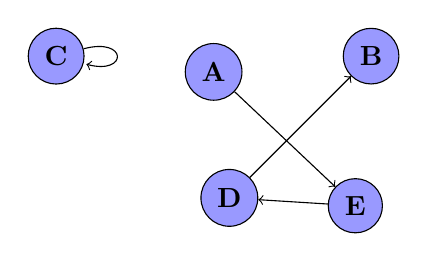
\begin{tikzpicture}
		\node[draw,circle,fill=blue!40!white](a) at (0,1.8) {\textbf{A}};
		\node[draw,circle,fill=blue!40!white](b) at (2,2) {\textbf{B}};
		\node[draw,circle,fill=blue!40!white](c) at (-2,2) {\textbf{C}};
		\node[draw,circle,fill=blue!40!white](d) at (0.2,0.2) {\textbf{D}};
		\node[draw,circle,fill=blue!40!white](e) at (1.8,0.1) {\textbf{E}};
		\draw[->] (a)--(e);
		\draw[->] (e)--(d);
		\draw[->] (d)--(b);
		\draw[->] (c) edge [loop right] ();
	\end{tikzpicture}
\end{document}
